\section{Относительность движения}

%1
\AddProb Два поезда движутся навстречу друг другу со скоростью $v$ каждый. 
Определите время встречи поездов, если начальное расстояние между ними равно $L$. 
Решите задачу координатным способом, графическим способом и методом, использующим идею относительности движения.
%\medskip

\AddProb Муха летает между двумя сближающимися со скоростью $v$ стенками. 
Скорость мухи $u$. Начальное расстояние между стенками равно $L$. 
Какой путь пройдет муха до остановки, если считать, что как только она приближается к одной из стенок -- мгновенно изменяет 
направление скорости на противоположное и движется вдоль одной прямой, перпендикулярной стенкам?

\AddProb Проплывая под мостом против течения, гребец потерял соломенную шляпу. 
Обнаружив пропажу через десять минут, он повернул назад и, гребя с тем же темпом, подобрал шляпу на расстоянии 900 м ниже моста. 
Через какое время после обнаружения пропажи гребец подобрал шляпу?

\AddProb С какой скорость должен двигаться автомобиль, чтобы капли дождя не оставляли следов на заднем стекле, 
наклоненном под углом $ \alpha $? Скорость дождя $\vec v$.

\AddProb Под каким углом к направлению течения должен плыть пловец, 
чтобы переправиться на противоположный берег с наименьшим смещением из-за течения реки? 
Скорость пловца $\vec u$, скорость реки $\vec v$.

%6
\AddProb Шарик движется навстречу стенке со скорость $\vec u$, скорость движения стенки $\vec v$. 
Определите, с какой скоростью отскочит шарик от стенки после абсолютно упругого удара. 
Как изменится ответ, если стенка движется в ту же строну, что и шарик? 
Если шарик падает под углом $ \alpha $ к стенке?

\AddProb Определите кратчайшее расстояние между автомобилями, которые движутся со скоростями $v$ по перпендикулярным пересекающимся прямым. 
В начальный момент времени один автомобиль находится в центре перекрестка, а второй подъезжает к нему на расстоянии $L$. 
Как изменится ответ, если угол между прямыми равен $ \alpha $ ?

\AddProb Как изменяется расстояние между двумя каплями воды, которые свободно падают в поле силы тяжести? 
Обе капли выпущены из одной точки с интервалом времени 1 секунда.

\AddProb Два тела движутся по прямой навстречу друг другу с начальными скоростями $\vec{v}_1$ и $\vec{v}_2$ и 
постоянными ускорениями $\vec{a}_1$ и $\vec{a}_2$, направленными противоположно соответствующим скоростям в начальный момент времени. 
При каком максимальном начальном расстоянии $L_{max}$ между телами они встретятся в процессе движения?

\AddProb Открытая карусель вращается с угловой скоростью $\omega $. На карусели на расстоянии $r$ от оси вращения стоит человек. 
Идет дождь, и капли дождя падают вертикально вниз со скоростью $v_0$. 
Как человек должен держать зонт, чтобы наилучшим образом укрыться от дождя?

%11
\AddProb От колеса радиуса $R$, движущегося без проскальзывания по горизонтальной поверхности со скоростью $\vec v$, 
отрывается вертикально кусочек грязи и, пролетев по воздуху, возвращается точно в ту же точку, от которой оторвался. 
При каких условиях это возможно?

\AddProb Маленький шарик, брошенный с начальной скоростью $\vec{v}_0$ под углом $\alpha$ к горизонту, 
ударился о вертикальную стенку, движущуюся ему навстречу с горизонтально направленной скоростью $\vec v$, и отскочил в точку, из которой был брошен. 
Определите, через какое время $t$ после броска произошло столкновение шарика со стенкой? Потерями на трение пренебречь.

\begin{wrapfigure}{r}{3.5cm}
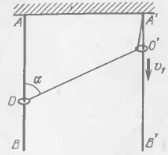
\includegraphics[width=3.5cm]{0113RelativityRings.jpg}
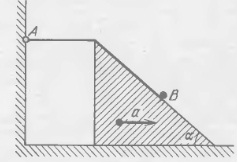
\includegraphics[width=3.5cm]{0114RelativityWedge.jpg}
\end{wrapfigure}

\AddProb Два колечка $O$ и $O'$ надеты на вертикальные неподвижные стержни $AB$ и $A'B'$ соответственно. 
Нерастяжимая нить закреплена в точке $A'$ и на колечке $O$ и продета через  колечко $O'$. 
Считая, что колечко $O'$ движется вниз с постоянной скоростью $\vec v$, определите скорость $\vec{v}_2$ колечка $O$, если  $\angle AOO' = \alpha$.

\AddProb На неподвижном клине, образующем угол $\alpha$  с горизонтом, лежит нерастяжимая невесомая веревка. 
Один из концов веревки прикреплен к стене в точке $A$. В точке $B$ к веревке прикреплен небольшой грузик. 
В некоторый момент времени клин начинает двигаться вправо с постоянным ускорением $\vec a$. 
Определите ускорение $\vec{a_{2}}$ грузика, пока он находится на клине.

\begin{wrapfigure}{r}{3.5cm}
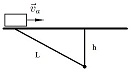
\includegraphics[width=3.5cm]{012011RelativityBus.jpg}
\end{wrapfigure}

\AddProb (2011)\footnote{Здесь и далее год в скобках означает, что данная задача была предложена для решения на Краевой студенческой олимпиаде
 по физике в Пермском крае в указанном году.}По шоссе со скоростью $\vec{v}_a$ движется автобус. Человек находится на расстоянии $h$ от шоссе и на расстоянии $L$ от автобуса. 
Под каким углом $\alpha$ к шоссе со скоростью $\vec v$  должен идти человек, чтобы выйти на шоссе одновременно с автобусом? 

%16
\AddProb (2009) Самолет в безветренную погоду взлетает со скоростью $\vec v$  под углом к горизонту $\alpha_0$ . 
Внезапно начинает дуть горизонтальный встречный ветер, скорость которого $\vec u$ . 
Какой стала скорость самолета относительно земли, и какой угол составляет она с горизонтом? 

\AddProb (2010) Когда мимо пристани проплывает плот, от пристани в деревню, расположенную на расстоянии $S$ вниз по течению реки, 
отправляется моторная лодка. Она доходит до деревни за время $t$ и, сразу повернув обратно, встречает плот на расстоянии $ S_1 $ от деревни. 
Какова скорость течения реки $\vec{v}_p $?

\AddProb (2013) Самолет садится на корабль, движущийся по океану со скоростью $\vec{v}_1$ в восточном направлении. 
Скорость ветра $\vec{v}_2$ направлена на север, а самолет снижается по отношению к кораблю вертикально со скоростью $\vec{v}_3$. 
Определить величину скорости самолета по отношению к движущемуся воздуху.

\begin{wrapfigure}{r}{3.5cm}
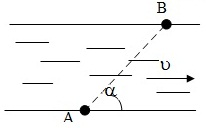
\includegraphics[width=3.5cm]{0115RelativityPowerboats.jpg}
\end{wrapfigure}

\AddProb (2007) Два катера вышли одновременно из пунктов $A$ и $B$, находящихся на противоположных берегах реки, и двигались вдоль отрезка $AB$ длины~$l$. 
Прямая $AB$ образует угол $\alpha$ с направлением скорости течения $\vec v$. Скорости движения катеров относительно воды одинаковы. 
На каком расстоянии от пункта $B$ произошла встреча катеров, если они встретились через время $t$ после отхода от причалов?